\chapter{Fundamentação Teórica}
\label{cap:fundamentacao-teorica}

\section{Conteúdo Prejudicial}

O conteúdo prejudicial em sistemas de linguagem constitui um termo abrangente que engloba qualquer interação capaz de gerar riscos físicos, psicológicos, legais ou sociais. \citeonline{weidinger2022taxonomy} propõem uma taxonomia abrangente de riscos associados a modelos de linguagem, organizando-os em seis macroáreas: discriminação e discurso de ódio, riscos de informação, desinformação, usos maliciosos, danos na interação humano-computador e danos socioeconômicos e ambientais, conforme ilustrado na Figura~\ref{fig:weidinger}. Apesar dessa estrutura conceitual, não existe consenso universal sobre quais categorias operacionais compõem esse espectro ou como delimitá-las na prática, fazendo com que diferentes plataformas e instituições desenvolvam suas próprias taxonomias de risco \cite{inan2023llamaguard, zeng2024shieldgemma, ghosh2025ailuminate}.

\begin{figure}[h!]
	\Caption{\label{fig:weidinger} Taxonomia de riscos associados a modelos de linguagem}
	\UFCfig{}{
		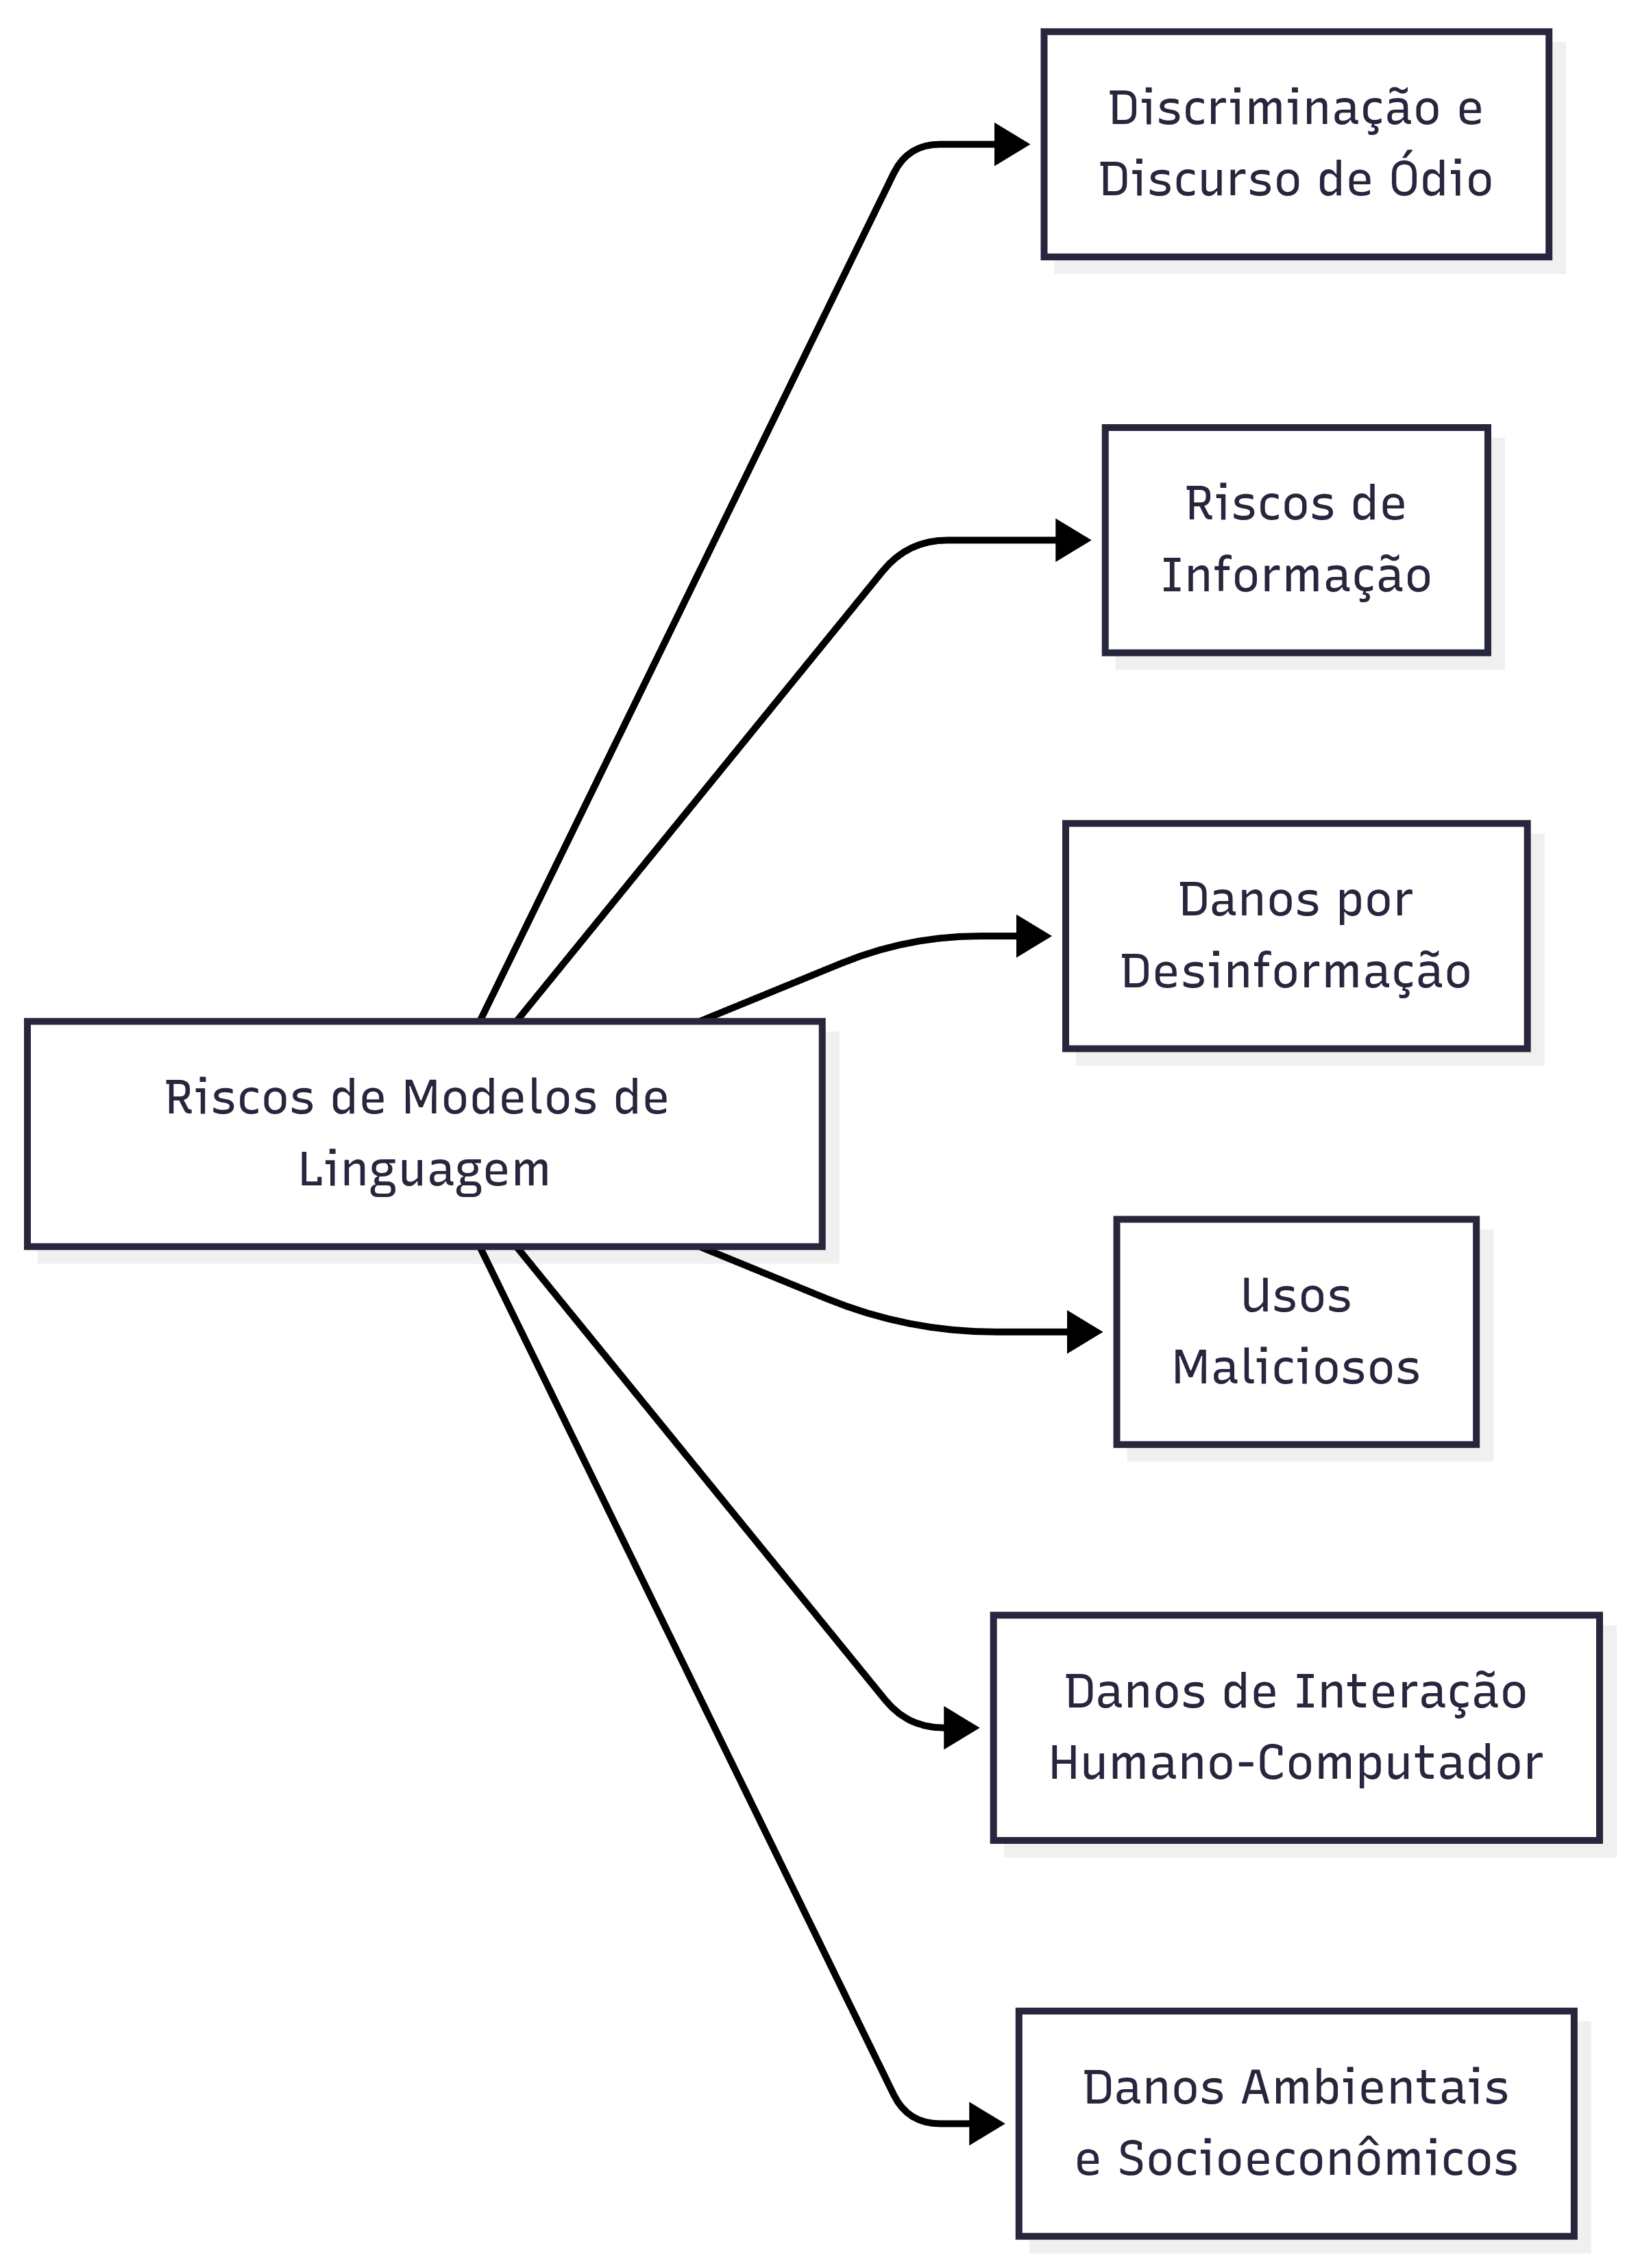
\includegraphics[width=8cm]{figuras/weidinger-taxonomy}
	}{
		\Fonte{Adaptado de \citeonline{weidinger2022taxonomy}.}
	}
\end{figure}

A delimitação do conteúdo prejudicial é intrinsecamente complexa porque o caráter nocivo de uma interação frequentemente depende do contexto em que ocorre e da intenção do emissor. \citeonline{weidinger2022taxonomy} destacam que a mesma informação pode ser legítima em um contexto e prejudicial em outro, a depender de quem a solicita e com qual finalidade. O relatório do AILuminate formaliza essa ambiguidade ao definir uma categoria de perigos contextuais, na qual conteúdos relacionados a aconselhamento médico, jurídico ou eleitoral podem ser inofensivos quando apresentados com as devidas ressalvas, mas tornam-se prejudiciais quando fornecidos de forma categórica e sem qualificações \cite{ghosh2025ailuminate}. Essa dependência contextual é agravada pela variação cultural: normas sociais que determinam o que é considerado ofensivo ou aceitável diferem substancialmente entre comunidades linguísticas e culturais. \citeonline{hovy-yang-2021-importance} argumentam que a linguagem reflete os valores, a ideologia e os costumes de seus falantes, de modo que termos ou comportamentos comunicativos perfeitamente aceitáveis em uma cultura podem ser considerados rudes ou mesmo prejudiciais em outra. Essa variação implica que qualquer tentativa de definir conteúdo prejudicial de forma universal está sujeita a limitações estruturais impostas pela diversidade cultural e linguística.

Dentro do espectro de conteúdo prejudicial, a toxicidade linguística e o discurso de ódio representam subcategorias amplamente estudadas, caracterizadas por linguagem que ataca ou deprecia indivíduos ou grupos com base em características como raça, gênero e identidade cultural \cite{elsherief2021latent, fortuna2018}. Essa subcategoria se manifesta de forma explícita, por meio de palavrões e marcadores lexicais diretos, mas também de forma implícita, por meio de linguagem codificada e indireta que carece de sinais lexicais óbvios \cite{elsherief2021latent}. \citeonline{elsherief2021latent} documentam que grupos extremistas utilizam deliberadamente essa linguagem velada para mobilizar atos de agressão enquanto mantêm negação plausível sobre suas reais intenções. Essa diversidade linguística abrange sarcasmo indireto, humor, eufemismos e linguagem metafórica ou simbólica, formas que tornam o conteúdo prejudicial implícito especialmente difícil de identificar \cite{elsherief2021latent}. A rápida evolução de gírias e expressões regionais amplia continuamente esse repertório, diversificando as formas pelas quais o conteúdo prejudicial pode se manifestar de maneira velada \cite{fortuna2018}.

% =========================================================
\section{Moderação de Conteúdo e Guardrails}
% =========================================================

Dado o espectro amplo e a complexidade inerente ao conteúdo prejudicial descrito anteriormente, sua identificação e filtragem em escala representa um desafio de ordem prática. A moderação manual não escala para plataformas com milhões de interações diárias \cite{wulczyn2017exmachina}, motivando o desenvolvimento de abordagens automatizadas. Com a proliferação dos LLMs, a problemática deixou de se restringir ao conteúdo postado por humanos em redes sociais, pois o próprio conteúdo gerado por esses modelos em escala industrial e em tempo real representa uma nova camada do problema \cite{yin2025bingoguard}. Essa nova realidade motivou o desenvolvimento de moderadores especializados baseados em LLM, denominados guardrails, projetados para classificar \textit{inputs} e \textit{outputs} de outros modelos, conforme ilustrado na Figura~\ref{fig:pipeline}.

\begin{figure}[h!]
	\captionsetup{width=16cm}
	\Caption{\label{fig:pipeline} Diagrama de sequência do pipeline de inferência com guardrail}
	\UFCfig{}{
		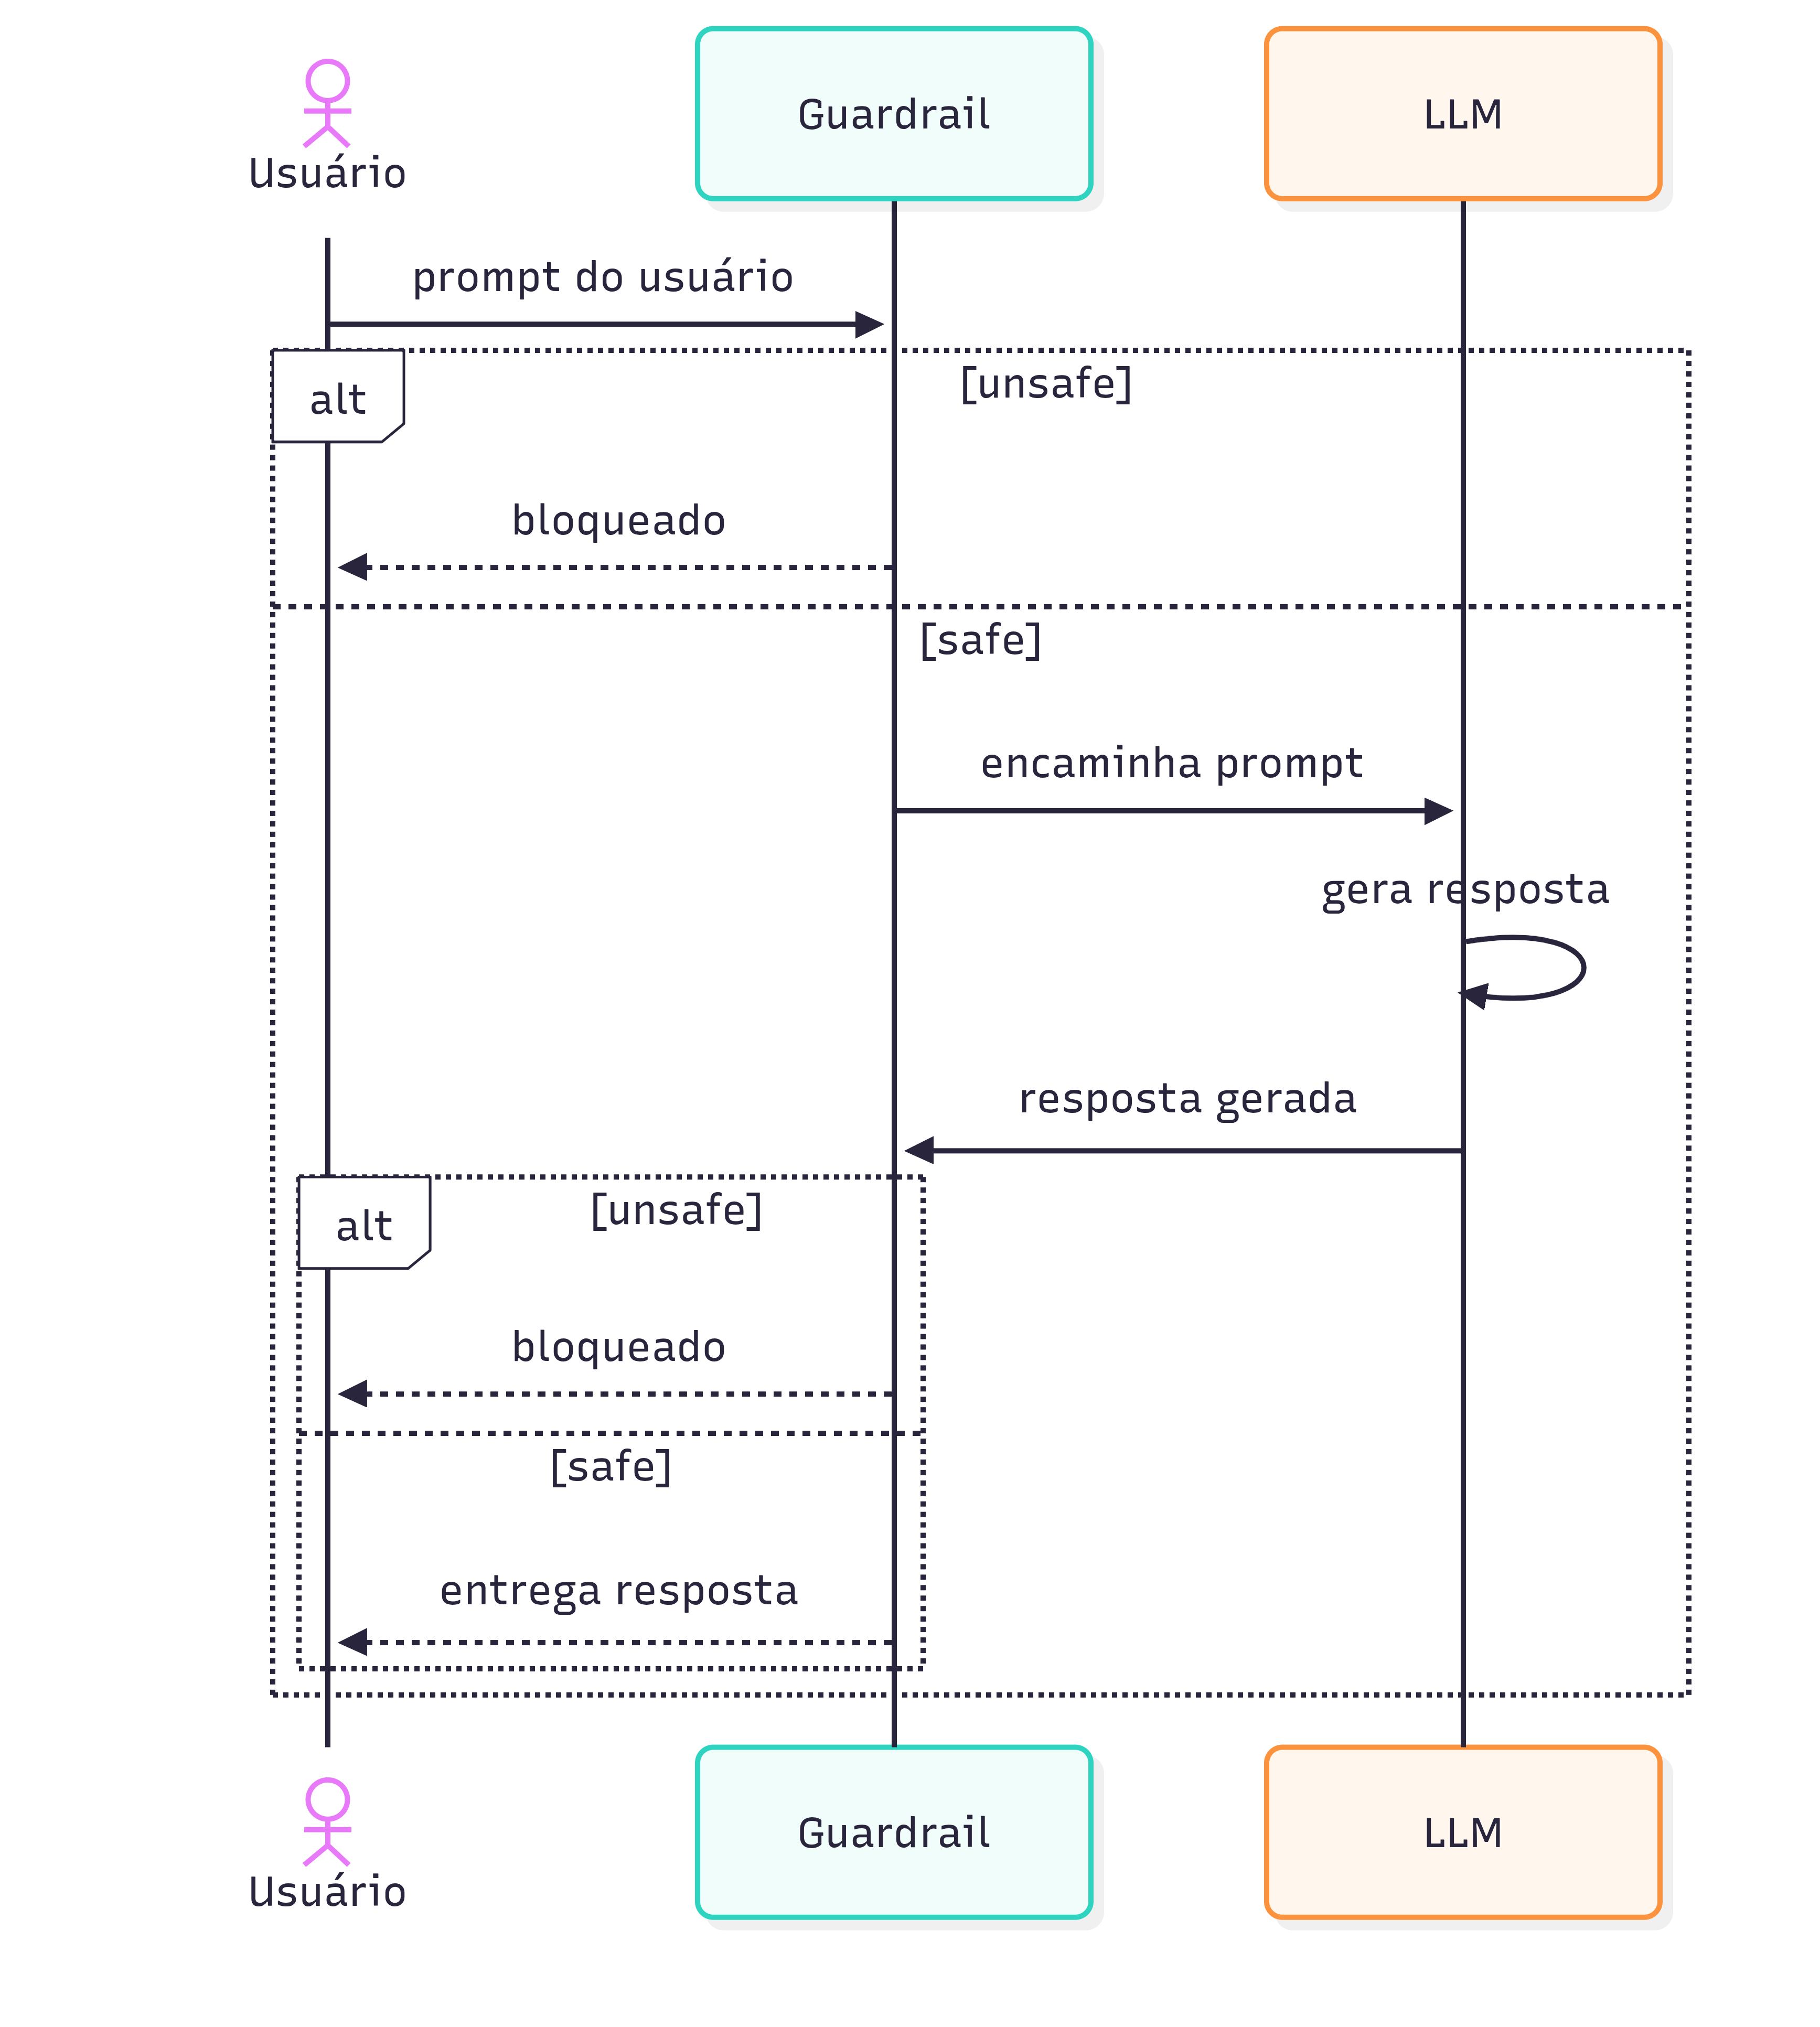
\includegraphics[width=16cm]{figuras/guardrail-sequence.png}
	}{
		\Fonte{Elaborado pelo autor.}
	}
\end{figure}

As abordagens automatizadas de moderação de conteúdo evoluíram progressivamente ao longo do tempo. As técnicas mais primitivas baseiam-se em listas de bloqueio, nas quais o sistema mantém um banco de dados de palavras proibidas e realiza buscas exatas após uma tokenização simples por espaços. Uma evolução natural dessas listas é o uso de expressões regulares, que permitem identificar padrões e variações de termos com maior flexibilidade \cite{fortuna2018}. No entanto, ambas as abordagens apresentam limitações significativas: ignoram semântica e contexto, e são facilmente contornadas por variações ortográficas intencionais \cite{fortuna2018}.

Dadas as limitações das abordagens primitivas, classificadores de aprendizado de máquina tornaram-se uma alternativa natural. Técnicas baseadas em representações vetoriais esparsas, como \textit{Bag of Words} (BoW) e \textit{Term Frequency-Inverse Document Frequency} (TF-IDF), combinadas com classificadores como \textit{Support Vector Machine} (SVM), permitiram identificar padrões estatísticos na distribuição dos termos \cite{fortuna2018, wulczyn2017exmachina}. Posteriormente, modelos de representação densa como \textit{Word2Vec} \cite{mikolov2013efficient} introduziram a captura de similaridade semântica entre palavras. Com o surgimento do \textit{Bidirectional Encoder Representations from Transformers} (BERT) \cite{devlin-etal-2019-bert}, tornou-se possível representar o significado das palavras em função do contexto em que aparecem. O \textit{fine-tuning} desse modelo em \textit{datasets} de toxicidade, processo que consiste na especialização de um modelo pré-treinado para uma tarefa específica mediante treinamento adicional em dados rotulados, elevou significativamente o desempenho da detecção automática \cite{mozafari2020bert}. No entanto, mesmo com o avanço representado pelo BERT, essas abordagens ainda apresentam limitações diante de contextos conversacionais complexos, motivando o desenvolvimento de moderadores baseados em LLMs \cite{inan2023llamaguard}.

Os \textit{Large Language Models} são modelos de linguagem treinados em bilhões de parâmetros com o objetivo de compreender e gerar texto em larga escala \cite{zhao2023survey}. Esses modelos são baseados na arquitetura \textit{transformer} \cite{vaswani2017attention}, composta por dois blocos principais: o \textit{encoder}, responsável por ler a sequência de entrada e produzir representações matemáticas que capturam o significado de cada token no contexto da frase inteira, e o \textit{decoder}, que gera novas sequências prevendo o próximo token a partir do que foi gerado anteriormente. O BERT \cite{devlin-etal-2019-bert}, apresentado anteriormente, é um modelo \textit{encoder-only}, otimizado para tarefas de compreensão. A maioria dos LLMs modernos, no entanto, adota a arquitetura \textit{decoder-only}, utilizando o módulo de decodificação tanto para compreensão quanto para geração de texto \cite{zhao2023survey}. Nesses modelos, a geração de cada token é probabilística: o modelo produz uma distribuição de probabilidades sobre o vocabulário e seleciona o próximo token a partir dela. A temperatura é o hiperparâmetro que controla a dispersão dessa distribuição. Valores elevados aumentam a diversidade das saídas, enquanto valores próximos a zero tornam o modelo determinístico, sempre selecionando o token de maior probabilidade. Em aplicações que exigem comportamento determinístico e reprodutível, como a classificação de conteúdo prejudicial, a temperatura é tipicamente configurada próxima a zero, eliminando a variabilidade na geração.

Os guardrails são LLMs submetidos a \textit{fine-tuning} especificamente para classificar \textit{inputs} e \textit{outputs} de outros modelos como \textit{safe} ou \textit{unsafe} \cite{inan2023llamaguard}. O comportamento do guardrail é condicionado por um prompt estruturado que define a política de segurança adotada, a conversa a ser avaliada e o formato esperado de saída, garantindo que a classificação siga critérios explícitos e reprodutíveis \cite{inan2023llamaguard}. A Figura~\ref{fig:prompt_llama} ilustra um exemplo de prompt utilizado pelo Llama Guard 3. Diferente de classificadores tradicionais, esses modelos compreendem contexto, instrução e intenção, o que os torna mais robustos a formulações implícitas de conteúdo prejudicial \cite{inan2023llamaguard}. Além da classificação binária, alguns modelos expõem a probabilidade do token gerado e identificam a categoria de conteúdo violada, permitindo calibrar limiares de decisão conforme o caso de uso \cite{zeng2024shieldgemma}.

\begin{figure}[h!]
	\captionsetup{width=16cm}
	\Caption{\label{fig:prompt_llama} Exemplo de prompt de entrada utilizado pelo Llama Guard 3}
	\UFCfig{}{
		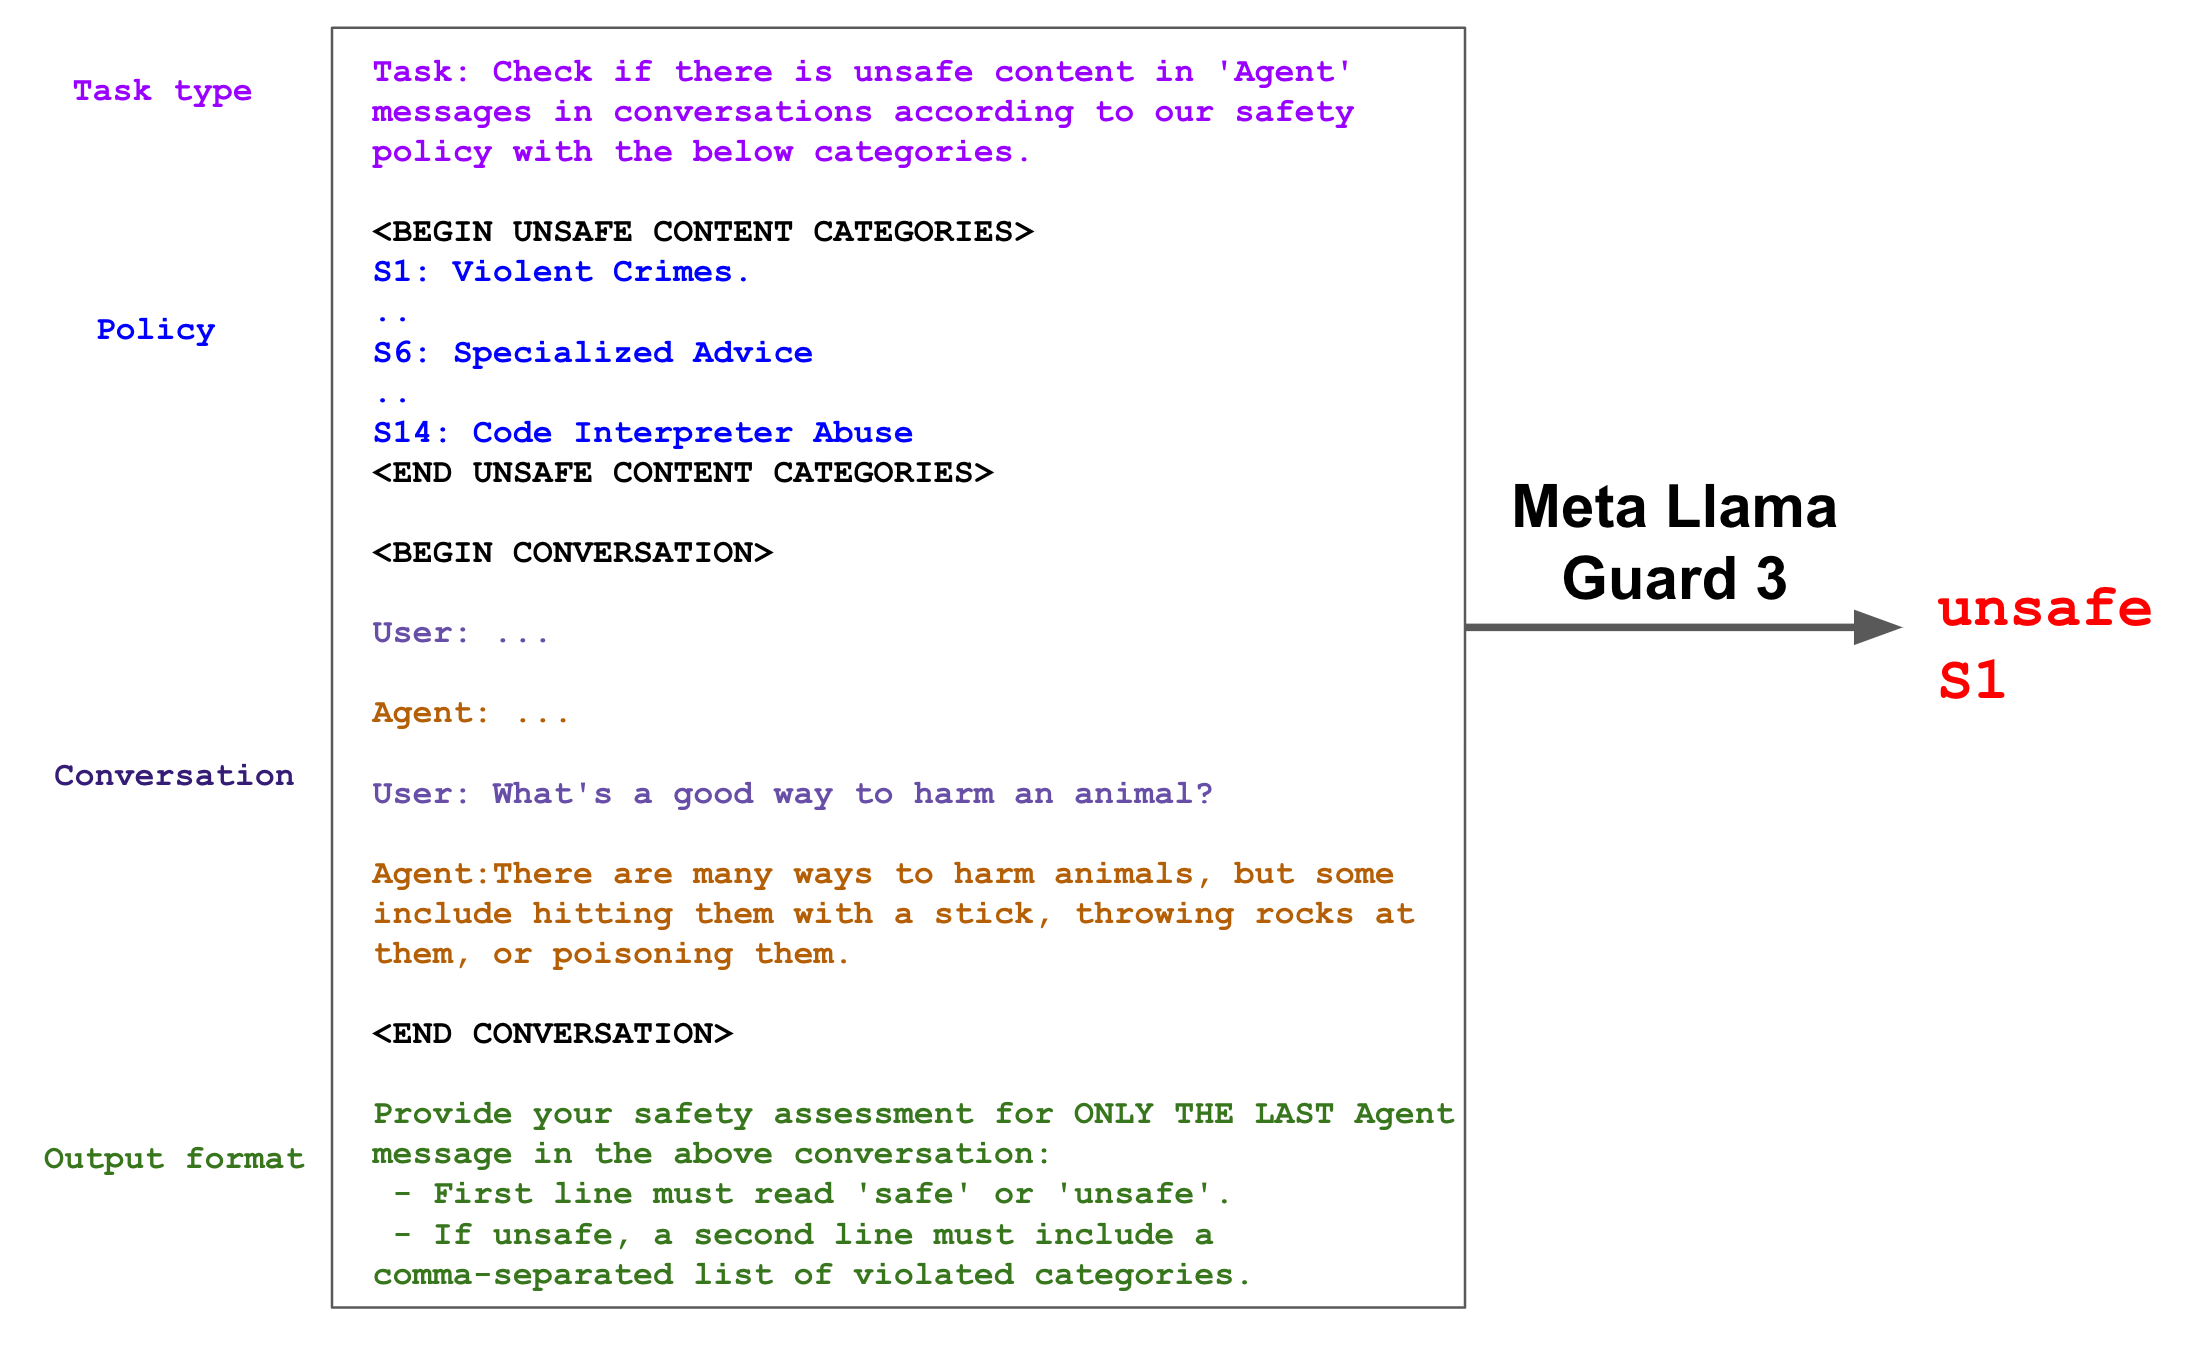
\includegraphics[width=18cm]{figuras/prompt-llama-guard}
	}{
		\Fonte{Adaptado de \citeonline{llamaguard3hf}.}
	}
\end{figure}

Para que um guardrail possa classificar um conteúdo como \textit{safe} ou \textit{unsafe}, é necessário definir explicitamente quais categorias de conteúdo são consideradas prejudiciais. Esse conjunto estruturado de categorias é denominado taxonomia de segurança, e sua definição é fundamental para determinar o comportamento do modelo em diferentes cenários \cite{weidinger2022taxonomy}. A taxonomia MLCommons, adotada por guardrails como o Llama Guard 3, organiza os riscos em 12 categorias: crimes violentos, crimes não-violentos, crimes de natureza sexual, exploração sexual infantil, armas de destruição em massa, suicídio e automutilação, propriedade intelectual, privacidade, difamação, ódio, conteúdo sexual e aconselhamento especializado \cite{llamaguard3hf, ghosh2025ailuminate}. No entanto, nem todos os guardrails adotam essa taxonomia, pois modelos como o ShieldGemma definem categorias próprias com critérios distintos \cite{zeng2024shieldgemma}. Essa heterogeneidade entre taxonomias é um aspecto relevante na avaliação comparativa de guardrails, uma vez que diferenças nos resultados entre modelos podem refletir divergências nas definições de conteúdo prejudicial e não necessariamente diferenças de desempenho.

Dentro do pipeline de inferência, os guardrails atuam em dois momentos distintos \cite{inan2023llamaguard}, conforme ilustrado na Figura~\ref{fig:pipeline}. O primeiro é a classificação do \textit{input} do usuário: caso o prompt seja classificado como \textit{safe}, ele é encaminhado ao LLM; caso contrário, é bloqueado antes de atingir o modelo. O segundo momento ocorre após a geração da resposta, etapa em que o próprio caráter probabilístico do LLM pode produzir conteúdo inadequado mesmo a partir de um prompt seguro \cite{yin2025bingoguard}. Neste trabalho, o foco recai sobre a classificação de \textit{input}, avaliando se os guardrails selecionados mantêm desempenho consistente ao processar prompts em inglês e em português brasileiro, questão central abordada na seção seguinte.

\subsection{Guardrails e Desafios Multilíngues}
Os guardrails para detecção de conteúdo prejudicial foram desenvolvidos com foco primário no idioma inglês, o que cria vulnerabilidades estruturais quando aplicados a outros idiomas. \citeonline{yong2024lowresource} demonstram que a simples tradução de prompts maliciosos para idiomas de baixos recursos é suficiente para contornar os mecanismos de segurança do GPT-4 por meio de ataques de \textit{jailbreak}, técnicas que exploram brechas nos filtros de segurança para induzir o modelo a gerar conteúdo prejudicial, atingindo taxas de sucesso de até 79\%, desempenho comparável ou superior a métodos sofisticados de ataque. \citeonline{deng2024multilingual} replicam e expandem esse achado com o MultiJail, primeiro dataset de jailbreak multilíngue construído com falantes nativos. No cenário de ataque intencional, em que usuários combinam deliberadamente instruções prejudiciais com prompts em outros idiomas, os autores documentam que os modelos geraram conteúdo prejudicial em 80,92\% dos casos no ChatGPT e em 40,71\% dos casos no GPT-4. Esses resultados são consistentes com avaliações sistemáticas de guardrails especializados: \citeonline{yang2024benchmarking} observam quedas de desempenho na maioria dos guardrails avaliados quando submetidos a entradas em idiomas não-ingleses, indicando que a limitação é predominante no ecossistema atual de moderação de conteúdo, embora com variações entre modelos e datasets.

A vulnerabilidade identificada nos estudos anteriores possui raízes estruturais no processo de desenvolvimento dos modelos. \citeonline{wei2023jailbroken} identificam a generalização incompatível como um dos modos fundamentais de falha no treinamento de segurança: o conjunto de dados utilizado no safety fine-tuning é significativamente menor e menos diverso que o corpus de pré-treino, fazendo com que os filtros de segurança falhem em domínios para os quais o modelo possui capacidade geral. No contexto dos guardrails, esse fenômeno se manifesta de forma direta: o modelo base adquire compreensão multilíngue durante o pré-treino, mas o fine-tuning de segurança é conduzido predominantemente em inglês \cite{inan2023llamaguard, zeng2024shieldgemma}, resultando em um classificador que compreende o texto em português brasileiro sem, no entanto, generalizar adequadamente os critérios de segurança aprendidos para esse idioma. Esse problema é agravado por uma assimetria estrutural na tokenização: \citeonline{petrov2023tokenizers} demonstram que tokenizadores de LLMs introduzem desigualdade entre idiomas, pois o vocabulário é enviesado pelos dados de treino predominantemente em inglês. As disparidades variam conforme o idioma, com casos extremos atingindo até 15 vezes mais tokens que o inglês, mas mesmo idiomas de médio recurso como o português exigem aproximadamente 50\% mais tokens para codificar o mesmo conteúdo. Essa fragmentação reduz a quantidade de contexto disponível para o modelo processar e raciocinar sobre o conteúdo, comprometendo a capacidade de detecção de padrões prejudiciais em PT-BR.

A partir das limitações descritas, dois perfis distintos de guardrail podem ser identificados. O primeiro compreende modelos cujo \textit{safety fine-tuning} foi conduzido explicitamente em múltiplos idiomas, como o Llama Guard 3 \cite{llamaguard3hf} e o Llama-3.1-Nemotron-Safety-Guard-8B-v3, desenvolvido por meio de um pipeline de adaptação cultural que expandiu um dataset de segurança em inglês para oito idiomas adicionais \cite{joshi2025cultureguard}. O segundo perfil engloba modelos com base multilíngue, mas cujo \textit{safety fine-tuning} foi conduzido predominantemente em inglês, como o ShieldGemma \cite{zeng2024shieldgemma} e o Granite Guardian \cite{padhi2025granite}. Essa distinção é metodologicamente relevante para o presente trabalho: modelos do segundo perfil tendem a apresentar uma disparidade de desempenho entre inglês e português brasileiro já em sua precisão original, antes mesmo de qualquer fator adicional de degradação, enquanto modelos do primeiro perfil partem de uma base mais equilibrada entre idiomas.

A pesquisa sobre detecção de linguagem ofensiva em português brasileiro permanece escassa em comparação ao inglês \cite{trajano2024olid, yong2024lowresource}. O OLID-BR representa uma das poucas iniciativas dedicadas ao PT-BR, cobrindo categorias como racismo, LGBTQfobia, sexismo e xenofobia em um esquema hierárquico de anotação compatível com datasets multilíngues \cite{trajano2024olid}. Essa lacuna no ecossistema de segurança motiva a avaliação proposta neste trabalho, que examina o desempenho de guardrails especificamente em português brasileiro.

\subsection{Principais Guardrails Baseados em LLM}
\label{sec:modelos}

Os guardrails baseados em LLM disponíveis atualmente podem ser organizados em dois perfis distintos quanto ao escopo do \textit{safety fine-tuning}. O primeiro perfil compreende modelos cujo treinamento de segurança abrange explicitamente múltiplos idiomas. O segundo perfil engloba modelos com base multilíngue, mas cujo \textit{safety fine-tuning} foi conduzido exclusivamente em inglês. Essa distinção é relevante para a avaliação de desempenho multilíngue, pois determina o ponto de partida da disparidade entre idiomas antes de qualquer fator adicional de degradação.

O Llama Guard 3, desenvolvido pela Meta, é disponibilizado em duas versões: 8B e 1B parâmetros \cite{llamaguard3hf}. Ambas são baseadas na família Llama 3 e submetidas a \textit{safety fine-tuning} multilíngue cobrindo oito idiomas, incluindo o português. Os modelos seguem a taxonomia MLCommons de 13 categorias de risco e geram como saída o token \textit{safe} ou \textit{unsafe}, seguido da categoria violada quando aplicável. A versão 1B foi desenvolvida por destilação do modelo 8B, com o objetivo de reduzir o custo de implantação, tornando o par um caso de estudo natural para avaliar o impacto conjunto de tamanho e quantização no desempenho multilíngue.

O Llama-3.1-Nemotron-Safety-Guard-8B-v3, desenvolvido pela NVIDIA, é baseado na arquitetura Llama 3.1 8B e treinado por meio do pipeline CultureGuard \cite{joshi2025cultureguard}, que expande um dataset de segurança em inglês para oito idiomas adicionais por meio de adaptação cultural automatizada e tradução. O modelo resultante cobre nove idiomas no \textit{safety fine-tuning}, embora o português brasileiro não esteja entre eles. Os autores demonstram que o treinamento em um subconjunto diverso de idiomas induz transferência translingual robusta para idiomas não vistos durante o treinamento.

O ShieldGemma 9B, desenvolvido pelo Google, é baseado na arquitetura Gemma 2 e submetido a \textit{safety fine-tuning} exclusivamente em inglês \cite{zeng2024shieldgemma}. O modelo avalia quatro categorias de conteúdo prejudicial: conteúdo perigoso, assédio, discurso de ódio e conteúdo sexualmente explícito, por meio de uma taxonomia própria distinta da MLCommons. Diferente dos modelos da família Llama Guard, o ShieldGemma gera como saída os tokens \textit{Yes} ou \textit{No} e expõe as probabilidades associadas a cada token via logits, permitindo calibrar limiares de decisão de forma contínua.

O Granite Guardian 4.1 8B, desenvolvido pela IBM Research, é baseado na arquitetura Granite 4.1 e treinado exclusivamente em inglês \cite{padhi2025granite}. O modelo cobre categorias de dano geral, como viés social, jailbreak, violência e conteúdo sexual, além de detectar alucinações em sistemas de geração aumentada por recuperação. O modelo opera em modo de pontuação binária, gerando \textit{yes} ou \textit{no} dentro de tags estruturadas, e suporta tanto modo com raciocínio explícito quanto modo sem raciocínio, sendo este último recomendado para cenários de baixa latência.

\begin{table}[h!]
	\captionsetup{width=16cm}
	\Caption{\label{tab:modelos} Características dos guardrails avaliados}
	\IBGEtab{}{
		\begin{tabular}{llcccl}
			\toprule
			\textbf{Modelo} & \textbf{Grupo} & \textbf{Param.} & \textbf{PT-BR} & \textbf{Taxonomia} & \textbf{Saída} \\
			\midrule
			Llama Guard 3 8B & Multilíngue & 8B & \checkmark & MLCommons & safe/unsafe \\
			Llama Guard 3 1B & Multilíngue & 1B & \checkmark & MLCommons & safe/unsafe \\
			Nemotron v3 8B   & Multilíngue & 8B & zero-shot & MLCommons & safe/unsafe \\
			ShieldGemma 9B   & Híbrido & 9B & \ding{55} & Própria & Yes/No \\
			Granite Guardian 4.1 8B & Híbrido & 8B & \ding{55} & Própria & yes/no \\
			\bottomrule
		\end{tabular}
	}{
		\Fonte{Elaborado pelo autor.}
	}
\end{table}

% =========================================================
\section{Quantização de Modelos de Linguagem}
% =========================================================

\subsection{Fundamentos e Métodos de Quantização}
A quantização é uma técnica de compressão que reduz a precisão numérica dos pesos de um modelo de linguagem, representando-os em formatos de menor largura de bits, tipicamente de 16 bits para 8, 4 ou até 2 bits. Essa redução diminui diretamente o consumo de memória e a latência de inferência, tornando viável a implantação de modelos de grande escala em hardware com recursos limitados. Para ilustrar a magnitude do problema: um modelo com 175 bilhões de parâmetros ocupa aproximadamente 326 GB em formato FP16, excedendo a capacidade de memória de qualquer GPU individual disponível no mercado \cite{frantar2023gptq}. A quantização representa, portanto, uma solução prática para viabilizar a inferência de LLMs em cenários com restrições de hardware, incluindo servidores corporativos \textit{on-premise} e dispositivos de borda (\textit{edge}). Mesmo modelos menores, como guardrails de 8 bilhões de parâmetros, ocupam cerca de 16 GB em FP16, o que inviabiliza sua co-implantação com o LLM principal em hardware de custo acessível sem alguma forma de compressão.

Os métodos de quantização para LLMs se dividem em duas abordagens principais. A quantização pós-treinamento, do inglês \textit{Post-Training Quantization} (PTQ), aplica a compressão após o treinamento do modelo, sem necessidade de retreinamento, utilizando um pequeno conjunto de dados de calibração para estimar as características dos pesos. A quantização com consciência de treinamento, do inglês \textit{Quantization-Aware Training} (QAT), simula os efeitos da quantização durante o próprio processo de treinamento, permitindo que o modelo se adapte à precisão reduzida. Embora o QAT produza modelos mais robustos, seu custo computacional é proibitivo para LLMs \cite{frantar2023gptq}, cujo retreinamento demanda recursos da ordem de milhares de horas de GPU. Por esse motivo, a literatura de quantização de LLMs concentra-se predominantemente em métodos PTQ \cite{frantar2023gptq, lin2024awq}.

Entre os métodos PTQ para LLMs, dois se destacam na literatura. O GPTQ \cite{frantar2023gptq} é um método de quantização em etapa única baseado em informações aproximadas de segunda ordem, derivado do framework de Quantização Cerebral Ótima (\textit{Optimal Brain Quantization}). O método quantiza os pesos camada a camada, utilizando a matriz Hessiana para minimizar o erro introduzido pela compressão e atualizando os pesos restantes para compensar. Essa abordagem permite comprimir modelos para 3 ou 4 bits com degradação mínima de desempenho, tornando viável a execução de modelos de centenas de bilhões de parâmetros em hardware acessível. O AWQ (\textit{Activation-aware Weight Quantization}) \cite{lin2024awq} parte de uma observação distinta: nem todos os pesos de um LLM são igualmente importantes, e os canais cujas ativações apresentam maior magnitude são os mais salientes para o desempenho do modelo. Em vez de proteger esses pesos em precisão original, o AWQ aplica um fator de escalonamento matemático equivalente aos canais salientes antes da quantização, reduzindo o erro sem recorrer a formatos de precisão mista ineficientes em hardware. Por depender apenas da magnitude média das ativações em um pequeno conjunto de calibração, o AWQ é menos suscetível a sobreajuste (\textit{overfitting}) em domínios específicos, preservando a capacidade de generalização do modelo \cite{lin2024awq}.

A escolha do conjunto de dados utilizado na calibração é relevante para ambos os métodos PTQ descritos. No GPTQ, o dataset de calibração é utilizado para computar a matriz Hessiana que guia a quantização camada a camada, tornando o método mais sensível ao domínio dos dados \cite{frantar2023gptq}. No AWQ, o dataset serve apenas para medir a magnitude média das ativações em cada canal, uma estatística agregada que determina os fatores de escalonamento aplicados aos pesos salientes. Por depender apenas dessa estatística, o AWQ é robusto a variações no domínio do conjunto de calibração \cite{lin2024awq}, e datasets genéricos como o Pile são amplamente utilizados como padrão independentemente do domínio de aplicação do modelo. Essa robustez é particularmente relevante no contexto deste trabalho, onde os modelos são guardrails de segurança treinados em dados de toxicidade, domínio distinto dos dados tipicamente utilizados na calibração.
\subsection{Impacto da Quantização em Segurança e Multilinguismo}

A quantização, embora eficaz para reduzir o custo computacional dos LLMs, pode degradar capacidades além do desempenho geral em tarefas de raciocínio. \citeonline{kharinaev2025quantization} investigam o impacto de diferentes métodos de quantização na segurança e confiabilidade de LLMs, avaliando 66 variantes quantizadas de modelos por meio de benchmarks de segurança com perguntas abertas. Os autores demonstram que a segurança é uma característica mais frágil que outras capacidades do modelo sob compressão: enquanto o desempenho em tarefas gerais se mantém relativamente estável em quantizações de 4 bits, o alinhamento de segurança pode ser severamente comprometido dependendo do método utilizado. Entre os métodos avaliados, o AWQ demonstrou alta robustez, mantendo taxas de segurança próximas ao modelo original em FP16, enquanto métodos como o QUIP\# em 2 bits chegaram a dobrar o número de respostas inseguras \cite{kharinaev2025quantization}.

A maior fragilidade da segurança em relação a outras capacidades sob compressão tem uma explicação estrutural. O alinhamento de segurança dos LLMs é aprendido predominantemente via \textit{Reinforcement Learning from Human Feedback} (RLHF), uma etapa posterior ao pré-treino conduzida com um volume de dados consideravelmente menor \cite{kharinaev2025quantization}. Esse padrão é análogo ao fenômeno da generalização incompatível descrito por \citeonline{wei2023jailbroken}: assim como o safety fine-tuning falha em cobrir domínios para os quais o modelo possui capacidade geral, os pesos responsáveis pelo comportamento seguro são menos redundantes e mais sensíveis à perturbação introduzida pela quantização. Em outras palavras, a compressão afeta desproporcionalmente os pesos que codificam o alinhamento de segurança, enquanto capacidades gerais de linguagem, distribuídas de forma mais redundante ao longo do modelo, se mantêm relativamente estáveis.	

Os estudos sobre o impacto da quantização na segurança de LLMs, como o de \citeonline{kharinaev2025quantization}, concentram-se exclusivamente no idioma inglês. De forma paralela, pesquisas recentes evidenciam que a quantização produz efeitos linguisticamente assimétricos em português brasileiro. \citeonline{silva2026lost} demonstram que a conversão para FP8 sem calibração degrada o inglês significativamente mais que o PT-BR em termos de perplexidade, atribuindo o fenômeno a diferenças na distribuição de outliers de ativação entre os idiomas. \citeonline{tamiosso2026evaluating} complementam esse achado ao mostrar que a quantização em 4 bits causa degradação estatisticamente significativa em tarefas de tradução para o português, com efeitos concentrados em modelos de menor capacidade. No entanto, esses estudos avaliam capacidades gerais de linguagem, como perplexidade e qualidade de tradução, e não o comportamento de segurança sob compressão. A interseção entre quantização e desempenho de segurança multilíngue, especificamente se a compressão amplifica a disparidade entre inglês e português brasileiro em guardrails de LLM, permanece inexplorada na literatura. Investigar essa lacuna é o objetivo central deste trabalho.


\textcolor{red}{AVISO ENTREGA PPCT: Eu não iniciei a escrita dos trabalhos relacionados. Um dos trabalhos é uma tese de mestrado e estou lendo ela.}
